Para este punto se desarrollaron nuevas instancias random distintas a las anteriores. Se realizaron nuevas experimentaciones para corroborar la performance y calidad de soluci\'on de cada heuristica

Un ejemplo de dichas instancias es el siguiente:

\vspace*{0.3cm} \vspace*{0.3cm}
  \begin{center}
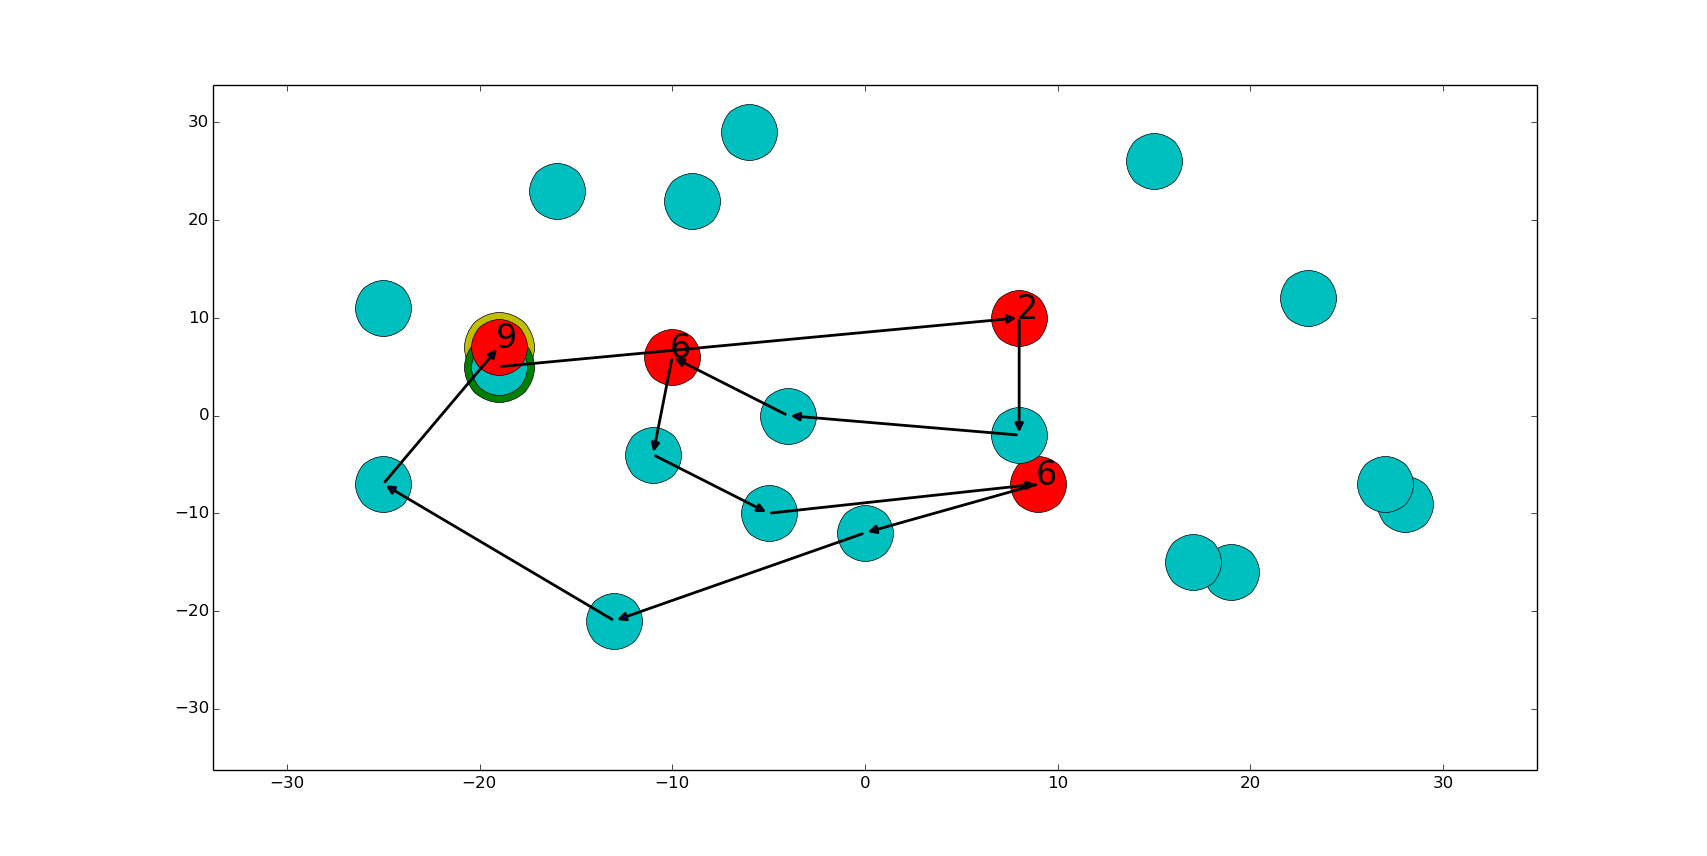
\includegraphics[scale=0.5]{./EJ5/caminoEjGoloso.png}
\\{\textit{Resultado goloso}}
  \end{center}
  \vspace*{0.3cm}
----> PONER UN GRAFICO DE BL Y OTRO DE TABU

\subsubsection{Comparaciones de performance entre heuristicas}

Para corroborar la performance obtenida para este grupo de instancias se tomaron los tiempos que tarda cada algoritmo en obtener soluci\'on.

Dicho conjunto esta formado por un total de 50 instancias que van desde 2 elementos hasta 50 en total.

-----> GRAFICO DE MEDICIONES 






\subsubsection*{Comparacion contra backtraking}
INSERTAR LA HEURISTICA MAS LENTA VS BACKTRACKING
\subsubsection{Comparacion de calidad de solución}
INSERTAR GRAFICOS DE BOXPLOTS ENTRE LOS ERRORES DE CADA HEURISTICA:
	ERROR VS TAMAÑO DE ENTRADA POR CADA HEURISTICA (cada columna que forme un boxplot en el grafico comparativo)
	